\chapter{INTRODUCTION AND CONTRIBUTIONS}
\label{chp:intro}
\blfootnote{Portions of this chapter have been submitted to:
  C.~W. Smith, B.~Granzow, G.~Diamond, D.~A. Ibanez, O.~Sahni, K.~E. Jansen
  \emph{et~al.}, ``In-memory integration of existing software components for
  parallel adaptive unstructured mesh workflows,'' submitted for publication.}

Unstructured mesh methods, like finite elements~\cite{hughes2012finite} or
finite volumes~\cite{abgrallFiniteVolume2016}, support the
effective analysis of complex physical behaviors modeled by partial differential
equations over general three-dimensional domains.
The most reliable and efficient methods apply adaptive procedures with \textit{a
posteriori} error estimators that indicate where and how the mesh is to be
modified.
Although adaptive meshes can have two to three orders of magnitude fewer
elements than a more uniform mesh for the same level of accuracy, there are many
complex simulations where the meshes required are so large that they can only be
solved on massively parallel systems.

The parallel simulations of interest are defined by a series of procedures which
we refer to as a workflow.
Fig.~\ref{fig:workflow} provides a high-level overview of this sequence.
Starting at the top-left the problem definition is specified on the
computational domain, typically a CAD model.
Next, automated mesh generation procedures driven by the problem definition and
optional mesh controls produce a spatial discretization of the computational
domain, a mesh.
With the mesh, the associated CAD model, and the problem definition, an analysis
is executed until some criterion is met that indicates adaptation is required.
In a workflow using mesh adaptation procedures this criterion is most effective
when it is based on the discretization error~\cite{hughes2012finite}.
Following the analysis, the adaptation procedure is executed to reduce the error
by locally refining and coarsening the mesh~\cite{li20053d,alauzet2006parallel}.
During these mesh modification operations local transfer
procedures~\cite{ibanezthesis} are executed to maintain an accurate
distribution of physical quantities of interest (e.g., the velocity of a fluid
or the displacement of a solid).
Once an adapted mesh has been created, the analysis procedure is executed again.
This solve-adapt cycle is repeated until a stopping criterion is met, such as a
pre-defined number of time/load steps.
After the last cycle completes, post-processing tools are executed to extract
spatial and temporal characteristics of the physical quantities of interest.

\begin{figure} \centering
  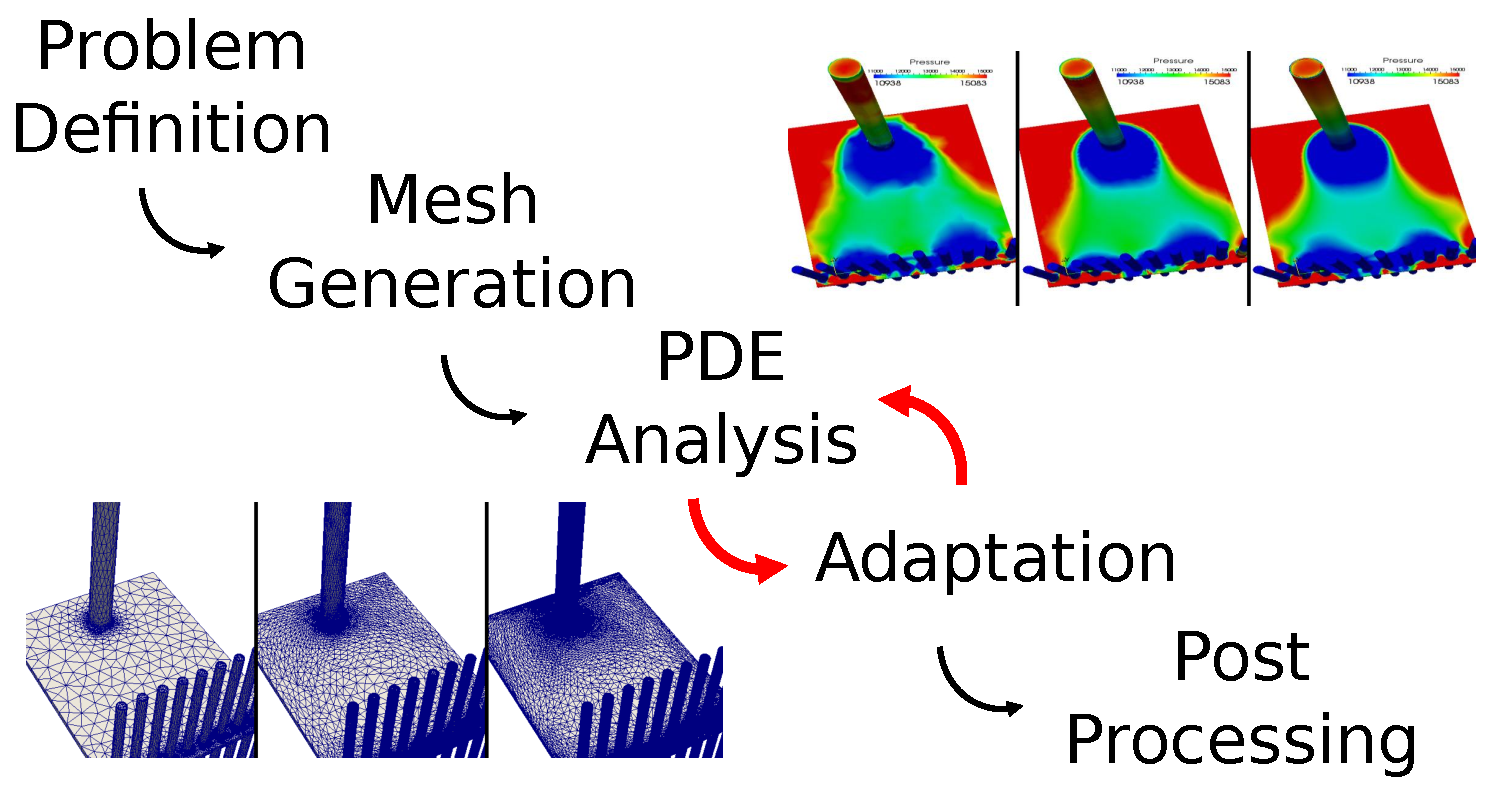
\includegraphics[width=.8\textwidth]{presentation/figs/SimulationBasedEngineeringWorkflow2.eps}
  \caption{
    The series of steps in an adaptive unstructured mesh-based workflow and
    (bottom) a sequence of adapted meshes and (top) the corresponding solution
    fields for an adaptive manifold flow
    simulation~\cite{ovcharenko2013parallel}.
  }
  \label{fig:workflow}
\end{figure}

The time spent running a parallel workflow is dominated by the repeated
execution of PDE analysis and adaptation procedures.
Efficiency of the analysis is maintained by redistributing the mesh after
adaptation procedures have non-uniformly refined and coarsened it.
Given an existing mesh distribution across the processes running on a parallel system,
a partition, dynamic load balancing methods determine which mesh elements should
be moved between processes to reduce the imbalance and communication costs.
For part counts numbering in the tens of thousands, multi-level methods
operating on the dual graph of the mesh are sufficient~\cite{karypis1999parallel}, 
but beyond this concurrency level these methods often fail due to memory usage
that increases significantly with process count~\cite{harlacherMortonSFCvsParmetis2012}.
The goal of \textbf{Par}titioning using \textbf{M}esh \textbf{A}djacencies (ParMA)
is to perform efficient, multi-criteria, dynamic load balancing of
unstructured meshes by directly using the existing mesh adjacency information.
Results will demonstrate the ability of ParMA to dynamically re-balance meshes
for multiple criteria with billions of mesh regions on over one million
processors.
Thus, ParMA addresses a key limitation to workflow scalability by enabling
efficient transformation of data within the computationally dominant analysis
procedures.

Within the solve-adapt cycle are transfers of mesh and field data between
analysis and adaptation procedures (depicted by the pair of bold arrows in
Fig.~\ref{fig:workflow}).
In massively parallel simulations requiring frequent adaptation, the reading and
writing of files between the execution of analysis and adaptation procedures
introduces significant computational overheads.
To avoid shared and contentious parallel filesystems, our in-memory coupling
approaches using data streams and APIs provide scalable and efficient transfers
of data by using node-local memory.
Thus, in-memory transfer approaches address a second key limitation to parallel
workflow scalability.

\section{Contributions}
The work of this thesis develops load balancing and in-memory workflow construction
methods for conformal 2D and 3D unstructured meshes composed of quadrilaterals,
triangles, tetrahedra, prisms, hexahedra, and pyramids.
A conformal mesh is one in which the intersection of two elements is a lower
order mesh entity shared by both (i.e., a face for two regions, an edge for two faces,
and a vertex for two edges).

\subsection{Dynamic Partition Improvement}
ParMA provides dynamic load balancing methods that compliment existing graph and
geometric partitioners to create mesh partitions with billions of elements
on millions of processors that are tailored to the needs of a given application.
Partition improvement results at various per part element counts on over one
million processors are discussed.

\subimport{parmaimprovement/}{parmaContributions}

\subsection{In-memory Component Coupling}
Critical to the construction of parallel workflows is the ability to couple existing
pieces of software.
We define bulk and atomic level couplings implemented using API- and data
stream-based approaches.
These in-memory couplings are applied to a monolithic, mixed C/C++ and FORTRAN,
computational fluid dynamics (CFD) analysis code, a C++, hp-adaptive, finite
element framework for linear accelerator frequency analysis, and a C++
multi-physics framework.
Scaling results up to 16,384 processes are provided for the coupling of the
massively parallel PHASTA CFD analysis code with mesh adaptation, and the memory
overhead for the linear accelerator framework when coupled with mesh adaptation
is studied.

\subsection{Parallel Workflows for Industrial Applications}
In addition to the three in-memory workflows discussed above, we also construct
parallel workflows for three industrial applications.
The first workflow demonstrates an adaptive, multi-phase flow simulation using an
in-memory coupling to a closed-source, serial procedure provided by the
industrial partner.
The second and third workflows focus on reducing the time engineers and analysts
have to spend setting up problems and running jobs by applying automation and
abstraction techniques.

\section{Thesis Organization}
The thesis is organized into the following chapters.
\begin{itemize}
  \item Chapter~\ref{chp:ptnImprovement} details the ParMA load balancing
    software and its support for extreme scale workflows.
  \item Chapter~\ref{chp:workflow} discusses the construction of parallel,
    unstructured mesh-based, in-memory workflows and the components that define
    them.
  \item Chapter~\ref{chp:inmem} describes the in-memory coupling for
    three unstructured mesh-based workflows and examines their performance
    relative to file-based approaches on massively parallel systems.
  \item Chapter~\ref{chp:hpcnyWorkflows} discusses three industrial workflows:
    one using in-memory coupling techniques, and two others using automation
    technologies.
  \item Chapter~\ref{chp:conclusion} summarizes the work and discusses some
    possible future efforts.
\end{itemize}

\section{Terminology and Notation}

\begin{tabular}{l|p{10cm}}
2D,3D              & two- and three-dimensional.\\
petascale,exascale & a computer system capable of executing $10^{15}$
                     and $10^{18}$ floating-point operations
                     per second, respectively.\\
CFD                & computational fluid dynamics.\\
CAE                & computer-aided engineering.\\
CAD                & computer-aided design/drafting.\\
ISV                & independent software vendor; typically a for-profit
                     organization with a closed-source product.\\
I/O                & input and output.\\
API                & application program interface.\\
CPU                & central processing unit; typically a socketed device
                     on the motherboard with multiple, independent, out-of-order
                     processing units.\\
(CPU) core         & a processing unit within a CPU.\\
GPU                & graphical processing unit; typically a bus-attached
                     device with thousands of group-synchronized, simple,
                     in-order processing units.\\
$O(1)$             & an operation that executes in constant time.\\
workflow           & the sequence of steps to set up and execute a
                     simulation.\\
(mesh) part        & a set of mesh elements and their closure assigned
                     to a given process.\\
(mesh) partition   & the set of parts forming a distributed mesh.\\
Ki                 & suffix to denote $2^{10}$. So, for example,
                     16Ki is equal to $16*2^{10} = 16384$.\\
$l.N$              & denotes the $N$th line of an Algorithm or
                     Listing.\\
\texttt{code}      & C/C++/Fortran is written with a fixed-pitch font.
                     For example, the function \texttt{printf(...)} is
                     declared in \texttt{stdio.h}; the ellipsis
                     represent omitted arguments.\\
\end{tabular}

\newpage

The following notation describes the topological entities of geometric models,
meshes, and partitions, the associations between the topological entities, and
the distribution of mesh entities in a partitioned mesh~\cite{ibanez2016pumi}.
\\

\begin{tabular}{l|p{10cm}}
$V$                         & the model, $V$ $\in$ \{$G$, $P$, $M$\}, where
                              $G$ is the geometric model, $P$
                              is the partition model, and $M$
                              is the mesh.
                              \\
$\{V^d\}$                   & the set of dimension $d$ entities in model $V$.\\
$V^d_i$                     & the $i^{th}$ entity of dimension $d$ in model
                              $V$.
                              $d=0$ for vertex, $d=1$ for edge, $d=2$ for
                              face, and $d=3$ for region.\\
\{$M^d_i$\{$M^q$\}\}        & a set of mesh entities of dimension $q$ that
                              are adjacent to $M^d_i$. For instance,
                              \{$M^1_3$\{$M^3$\}\} is a set of mesh regions
                              adjacent to mesh edge $M^1_3$. \\
$M^{d}_i \sqsubset G^{q}_j$ & the geometric classification indicating the
                              unique association of mesh entity $M^{d}_i$
                              with geometric model entity
                              $G^{q}_j$, $d \le q$.\\
$M^{d}_i \sqsubset P^{q}_j$ & the partition classification indicating the
                              unique association of mesh entity $M^{d}_i$
                              with partition model entity
                              $P^{q}_j$, $d \le q$.\\
$w_p(M^d)$                  & the weight of mesh entities $M^d$ on part $p$.\\
$I^d_p$                     & the weighted imbalance of dimension $d$ mesh entities
                              on part $p$;
                              $w_p(M^d_i) / avg(w_{q=0..N-1}(M^d_i))$
                              where $N$ is the total number of parts in the
                              mesh.\\
$I^d$                       & the maximum imbalance of entity dimension $d$;
                              $max(I^d_{p=0..N-1})$.
\end{tabular}
